\documentclass[main.tex]{subfiles}

\begin{document}

\section{Scalability of Original Implementation} \label{sec:results:original}

Since the code being used here was not subject to any intervention in terms of optimization, any performance issues with this version should not be directly associated with algorithm or hardware limitations, as code quality is not guaranteed.

It should also be noted that the SPPMPA version of this code was not fully finished at this time, so profiling of this original implementation was limited to the more basic PPM version. Regardless, the actual implementation of each task remained unchanged, and a good overview of the algorithm's scalability is still possible. The major drawback is that it becomes impossible to assess performance with concurrent iterations, which are not supported by PPM.

For these tests, three different computational systems were used, particular the 511, 611 and 711 nodes described in \cref{section:results:env}

Testing focused on the scalability of the algorithm on each of these nodes, by running 10 photon mapping iterations on each different scene.

\begin{figure}[!htp]
  \centering
  \begin{subfigure}{.5\textwidth}
    \centering
    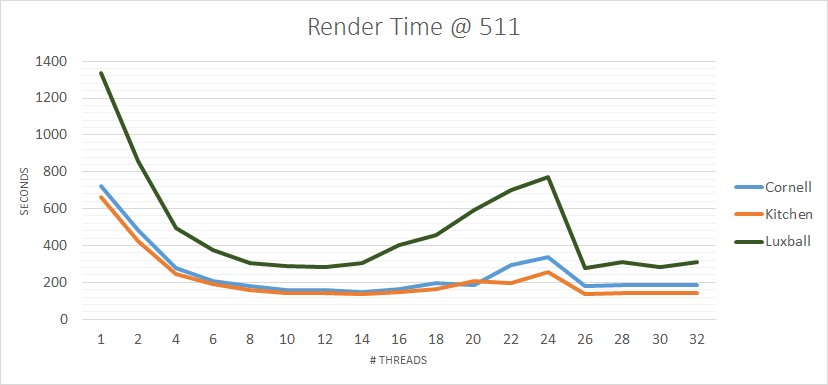
\includegraphics[width=\linewidth]{excel/rr_cpu_time_511}
    \caption{node 511 \label{fig:rr_cpu_time_511}}
  \end{subfigure}%
  \begin{subfigure}{.5\textwidth}
    \centering
    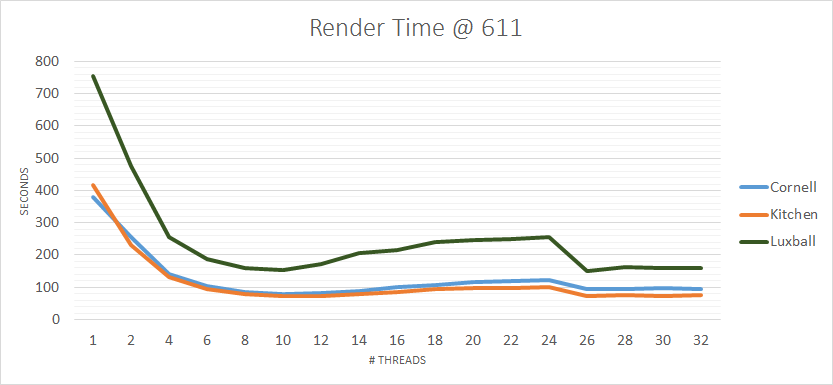
\includegraphics[width=\linewidth]{excel/rr_cpu_time_611}
    \caption{node 611 \label{fig:rr_cpu_time_611}}
  \end{subfigure}
  \caption{Original Implementation (\cpu only): Render time for 10 photon mapping iterations \label{fig:rr_cpu_time}}
\end{figure}

With these results, it can be noticed that peak performance is achieved when using around 12 \openmp threads for both the 511 and the 611 machines, although the performance is nearly identical when using more than 24 threads. This means that once the 511 machine uses up all of its cores, performance starts to drop, while for the 611 machine this only happens when both sockets (which possess only 6 cores each) are filled. This is more noticeable in \cref{fig:rr_cpu_speedup} which shows speedup versus sequential time, rather than global execution time.

\begin{figure}[!htp]
  \centering
  \begin{subfigure}{.5\textwidth}
    \centering
    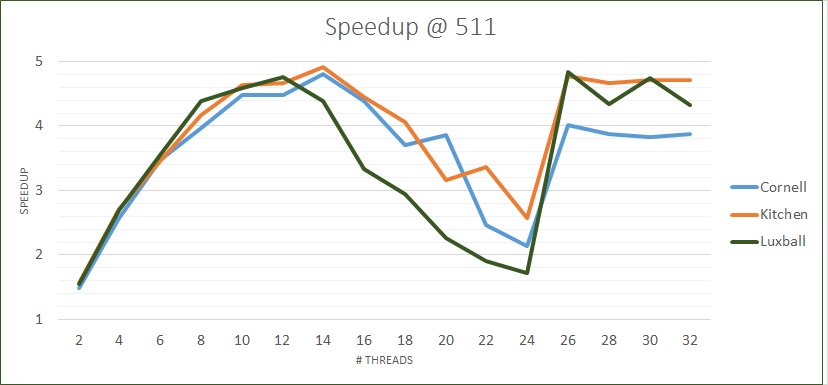
\includegraphics[width=\linewidth]{excel/rr_cpu_speedup_511}
    \caption{node 511 \label{fig:rr_cpu_speedup_511}}
  \end{subfigure}%
  \begin{subfigure}{.5\textwidth}
    \centering
    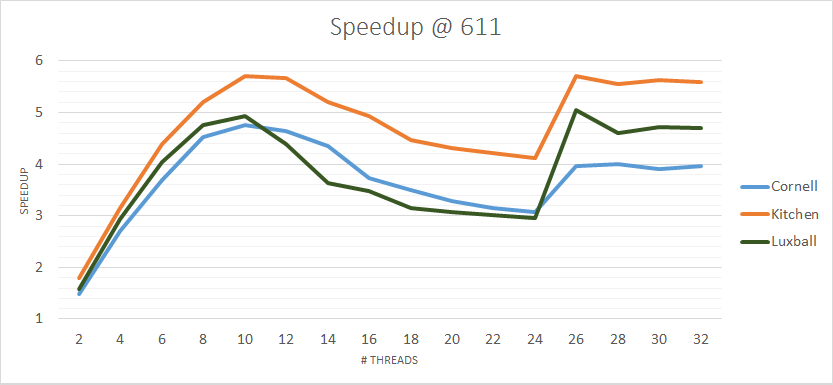
\includegraphics[width=\linewidth]{excel/rr_cpu_speedup_611}
    \caption{node 611 \label{fig:rr_cpu_speedup_611}}
  \end{subfigure}
  \caption{Original Implementation (\cpu only): Speedup for 10 photon mapping iterations \label{fig:rr_cpu_speedup}}
\end{figure}

\end{document}
